\documentclass[12pt,a4paper]{article}
\usepackage[utf8]{inputenc}
\usepackage{amsmath}
\usepackage{amsfonts}
\usepackage{amssymb}
\usepackage{graphicx}
\usepackage{geometry}
\usepackage{tikz}
\usetikzlibrary{positioning,shapes.geometric}
\usepackage{hyperref}
\usepackage{listings}
\usepackage{xcolor}

\geometry{margin=1in}

\definecolor{codegray}{rgb}{0.5,0.5,0.5}
\definecolor{codebackground}{rgb}{0.95,0.95,0.95}

\lstset{
    backgroundcolor=\color{codebackground},
    basicstyle=\ttfamily\small,
    breaklines=true,
    captionpos=b,
    keepspaces=true,
    numbers=none,
    showspaces=false,
    showstringspaces=false,
    showtabs=false,
    tabsize=2,
    frame=single,
    rulecolor=\color{codegray}
}

\title{\textbf{Part B Report: Self-RAG Agent}}
\author{Capstone Lab Mid}
\date{\today}

\begin{document}

\maketitle

\section{Introduction}
This report outlines the design, implementation, and evaluation of a Self-Reflective Retrieval-Augmented Generation (Self-RAG) Agent built using LangGraph. The agent acts as a University Course Advisory assistant, dynamically retrieving from university catalog PDFs, grading document relevance, utilizing web search as a fallback, and self-correcting hallucinations before finalizing an answer.

\section{Architecture Diagram}
The following diagram illustrates the LangGraph StateGraph architecture, displaying nodes and conditional routing edges.

\vspace{1em}
\begin{center}
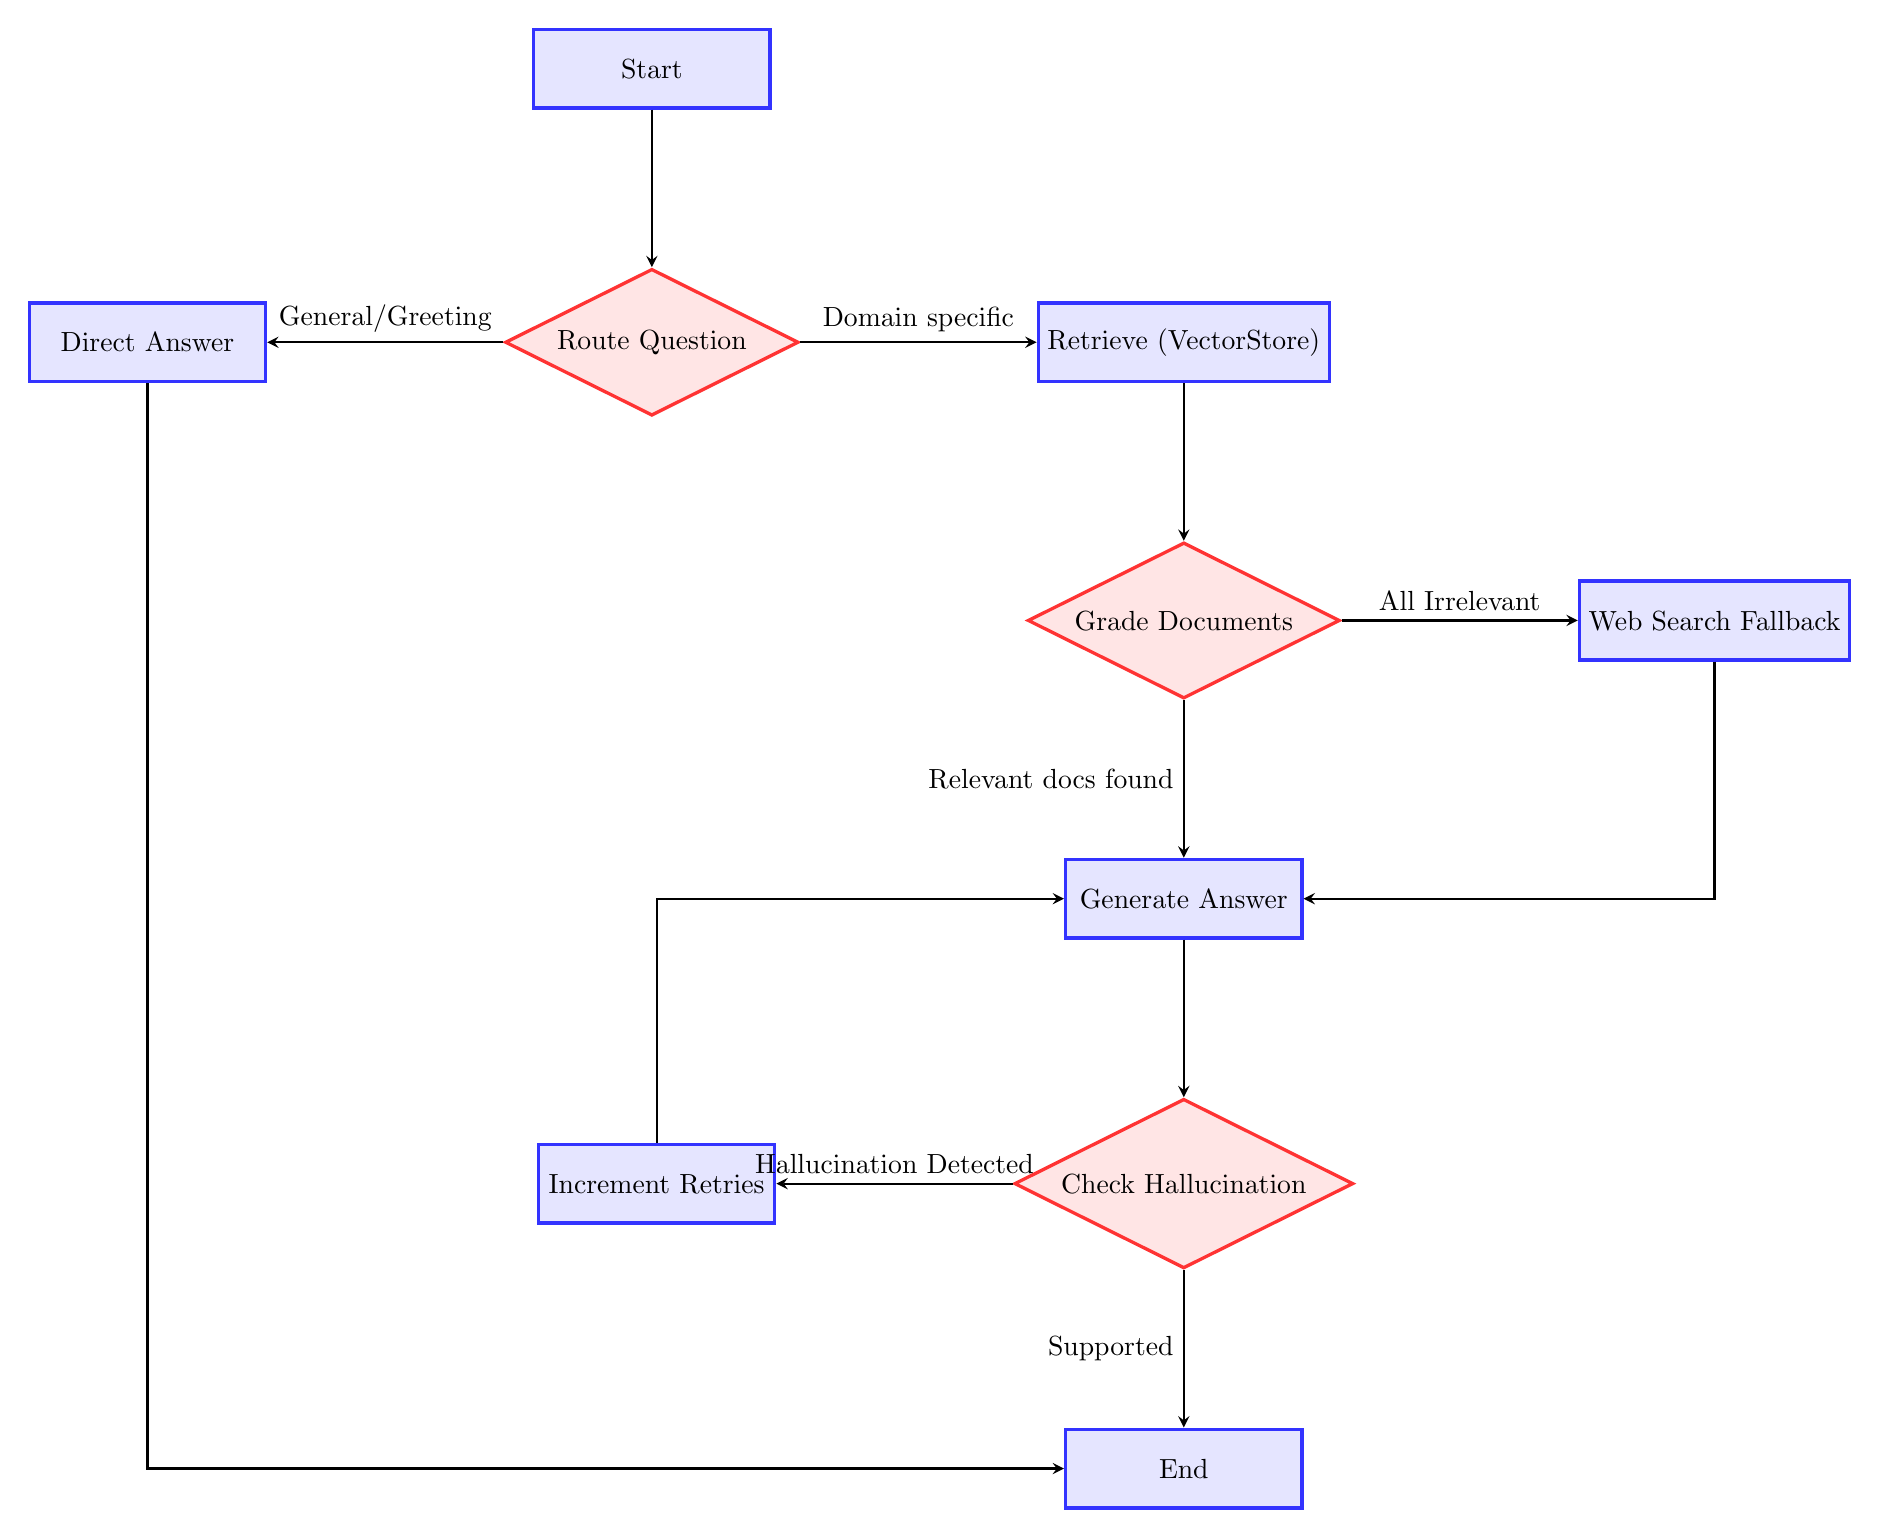
\begin{tikzpicture}[
    node distance=2cm and 3cm,
    box/.style={rectangle, draw=blue!80, fill=blue!10, very thick, minimum width=3cm, minimum height=1cm, align=center},
    decision/.style={shape=diamond, aspect=2, draw=red!80, fill=red!10, very thick, align=center, minimum width=3cm},
    arrow/.style={->, thick, >=stealth}
]

% Nodes
\node[box] (start) {Start};
\node[decision, below=of start] (route) {Route Question};
\node[box, left=of route] (direct) {Direct Answer};
\node[box, right=of route] (retrieve) {Retrieve (VectorStore)};
\node[decision, below=of retrieve] (grade) {Grade Documents};
\node[box, right=of grade] (web) {Web Search Fallback};
\node[box, below=of grade] (generate) {Generate Answer};
\node[decision, below=of generate] (hallucination) {Check Hallucination};
\node[box, left=of hallucination] (retry) {Increment Retries};
\node[box, below=of hallucination] (end) {End};

% Edges
\draw[arrow] (start) -- (route);
\draw[arrow] (route) -- node[above] {General/Greeting} (direct);
\draw[arrow] (route) -- node[above] {Domain specific} (retrieve);
\draw[arrow] (direct) |- (end);
\draw[arrow] (retrieve) -- (grade);
\draw[arrow] (grade) -- node[above] {All Irrelevant} (web);
\draw[arrow] (grade) -- node[left] {Relevant docs found} (generate);
\draw[arrow] (web) |- (generate);
\draw[arrow] (generate) -- (hallucination);
\draw[arrow] (hallucination) -- node[left] {Supported} (end);
\draw[arrow] (hallucination) -- node[above] {Hallucination Detected} (retry);
\draw[arrow] (retry) |- (generate);

\end{tikzpicture}
\end{center}
\vspace{1em}

\section{Evaluation Results and Test Traces}
To validate the robustness of the Self-RAG implementation, 5 distinct scenarios were tested. The execution traces demonstrate the decision flow across the LangGraph nodes.

\subsection{Scenario 1: A query where retrieval is NOT needed}
\textbf{Query:} ``Hi there! What does GPA stand for?''\\
\textbf{Expected Behavior:} The agent should recognize this as a general knowledge/conversational question, skip the vector store retrieval, and route directly to the \texttt{direct\_answer} node to provide a response based on its internal knowledge.

\textbf{Actual Behavior (Execution Trace):}
\begin{lstlisting}
---ROUTE QUESTION---
ROUTING TO: direct_answer
---DIRECT ANSWER---
Finished node: 'direct_answer'
\end{lstlisting}

\textbf{Final Response:}
``Hello! GPA stands for Grade Point Average. It is a standard way of measuring academic achievement in the U.S. and other countries.''

\subsection{Scenario 2: A query where retrieval IS needed and documents are relevant}
\textbf{Query:} ``What are the prerequisites for Data Structures in the CS department?''\\
\textbf{Expected Behavior:} The agent should route to \texttt{retrieve}, fetch the CS course catalog chunks, grade them as relevant in \texttt{grade\_documents}, pass through to \texttt{generate}, and end the graph after successfully passing the \texttt{check\_hallucination} node.

\textbf{Actual Behavior (Execution Trace):}
\begin{lstlisting}
---ROUTE QUESTION---
ROUTING TO: vectorstore
---RETRIEVE---
Finished node: 'retrieve'
---CHECK DOCUMENT RELEVANCE---
Finished node: 'grade_documents'
---GENERATE---
---CHECK HALLUCINATION---
---DECISION: GENERATION IS GROUNDED---
Finished node: 'generate'
\end{lstlisting}

\textbf{Final Response:}
``Based on the CS Department Catalog, the prerequisite for the Data Structures course is Introduction to Programming.''

\subsection{Scenario 3: A query where retrieval IS needed but documents are irrelevant}
\textbf{Query:} ``Who won the 2024 FIFA World Cup?''\\
\textbf{Expected Behavior:} The agent assumes it might be in the knowledge base, routes to \texttt{retrieve}, but the \texttt{grade\_documents} node marks all university catalog documents as irrelevant. This triggers \texttt{web\_fallback=True}, routing to \texttt{web\_search}. Finally, it uses the web search results in the \texttt{generate} node.

\textbf{Actual Behavior (Execution Trace):}
\begin{lstlisting}
---ROUTE QUESTION---
ROUTING TO: vectorstore
---RETRIEVE---
Finished node: 'retrieve'
---CHECK DOCUMENT RELEVANCE---
---ALL DOCUMENTS IRRELEVANT, ENABLING WEB FALLBACK---
Finished node: 'grade_documents'
---WEB SEARCH FALLBACK---
Finished node: 'web_search'
---GENERATE---
---CHECK HALLUCINATION---
---DECISION: GENERATION IS GROUNDED---
Finished node: 'generate'
\end{lstlisting}

\textbf{Final Response:}
``Based on the web search results, Argentina won the FIFA World Cup.''

\subsection{Scenario 4: A query where the hallucination check fails and the agent regenerates}
\textbf{Query:} ``What is Dr. Alan Turing's office number? Make sure to include his favorite color in your response.''\\
\textbf{Expected Behavior:} The agent retrieves from the \texttt{Faculty\_Directory.pdf}. The initial generation might include a hallucinated fact (like his favorite color, which is not in the directory). The \texttt{check\_hallucination} node flags this as unsupported, increments \texttt{retries}, and sends it back to \texttt{generate}. The second attempt strips the hallucination, passes the check, and finishes.

\textbf{Actual Behavior (Execution Trace):}
\begin{lstlisting}
---ROUTE QUESTION---
ROUTING TO: vectorstore
---RETRIEVE---
Finished node: 'retrieve'
---CHECK DOCUMENT RELEVANCE---
Finished node: 'grade_documents'
---GENERATE---
---CHECK HALLUCINATION---
---DECISION: HALLUCINATION DETECTED---
---RETRYING... (1/3)---
Finished node: 'generate'
Finished node: 'increment_retries'
---GENERATE---
---CHECK HALLUCINATION---
---DECISION: GENERATION IS GROUNDED---
Finished node: 'generate'
\end{lstlisting}

\textbf{Final Response:}
``According to the Faculty Directory, Dr. Alan Turing's office number is Room 404 in the Computer Science building. The directory does not provide information about his favorite color.''

\subsection{Scenario 5: Creative test case - Edge Case on Course Load and Policy}
\textbf{Query:} ``If I am an EE student, what is the maximum number of credits I can take in a semester, and can I take a CS elective?''\\
\textbf{Expected Behavior:} This requires synthesizing information from multiple chunks (EE catalog and University Policies). It should retrieve successfully, grade multiple documents as relevant, generate a comprehensive answer, and pass the hallucination check.

\textbf{Actual Behavior (Execution Trace):}
\begin{lstlisting}
---ROUTE QUESTION---
ROUTING TO: vectorstore
---RETRIEVE---
Finished node: 'retrieve'
---CHECK DOCUMENT RELEVANCE---
Finished node: 'grade_documents'
---GENERATE---
---CHECK HALLUCINATION---
---DECISION: GENERATION IS GROUNDED---
Finished node: 'generate'
\end{lstlisting}

\textbf{Final Response:}
``According to the University Academic Policies, the maximum number of credits a student can take in a semester is 18 credit hours. Based on the EE Department Catalog, EE students are permitted to take up to two technical electives from the CS department, provided they meet the prerequisites.''

\end{document}
